\label{sec:chi2}
%%%%%%%%%%%
In this section various forms of $\chi^2$ are described, 
based on the use of nuisance parameters or on th full covariance matrix.
A schematic picture of $\chi^2$ definitions is displayed in Fig. \ref{fig:chi2}.
\begin{figure}
\begin{center}
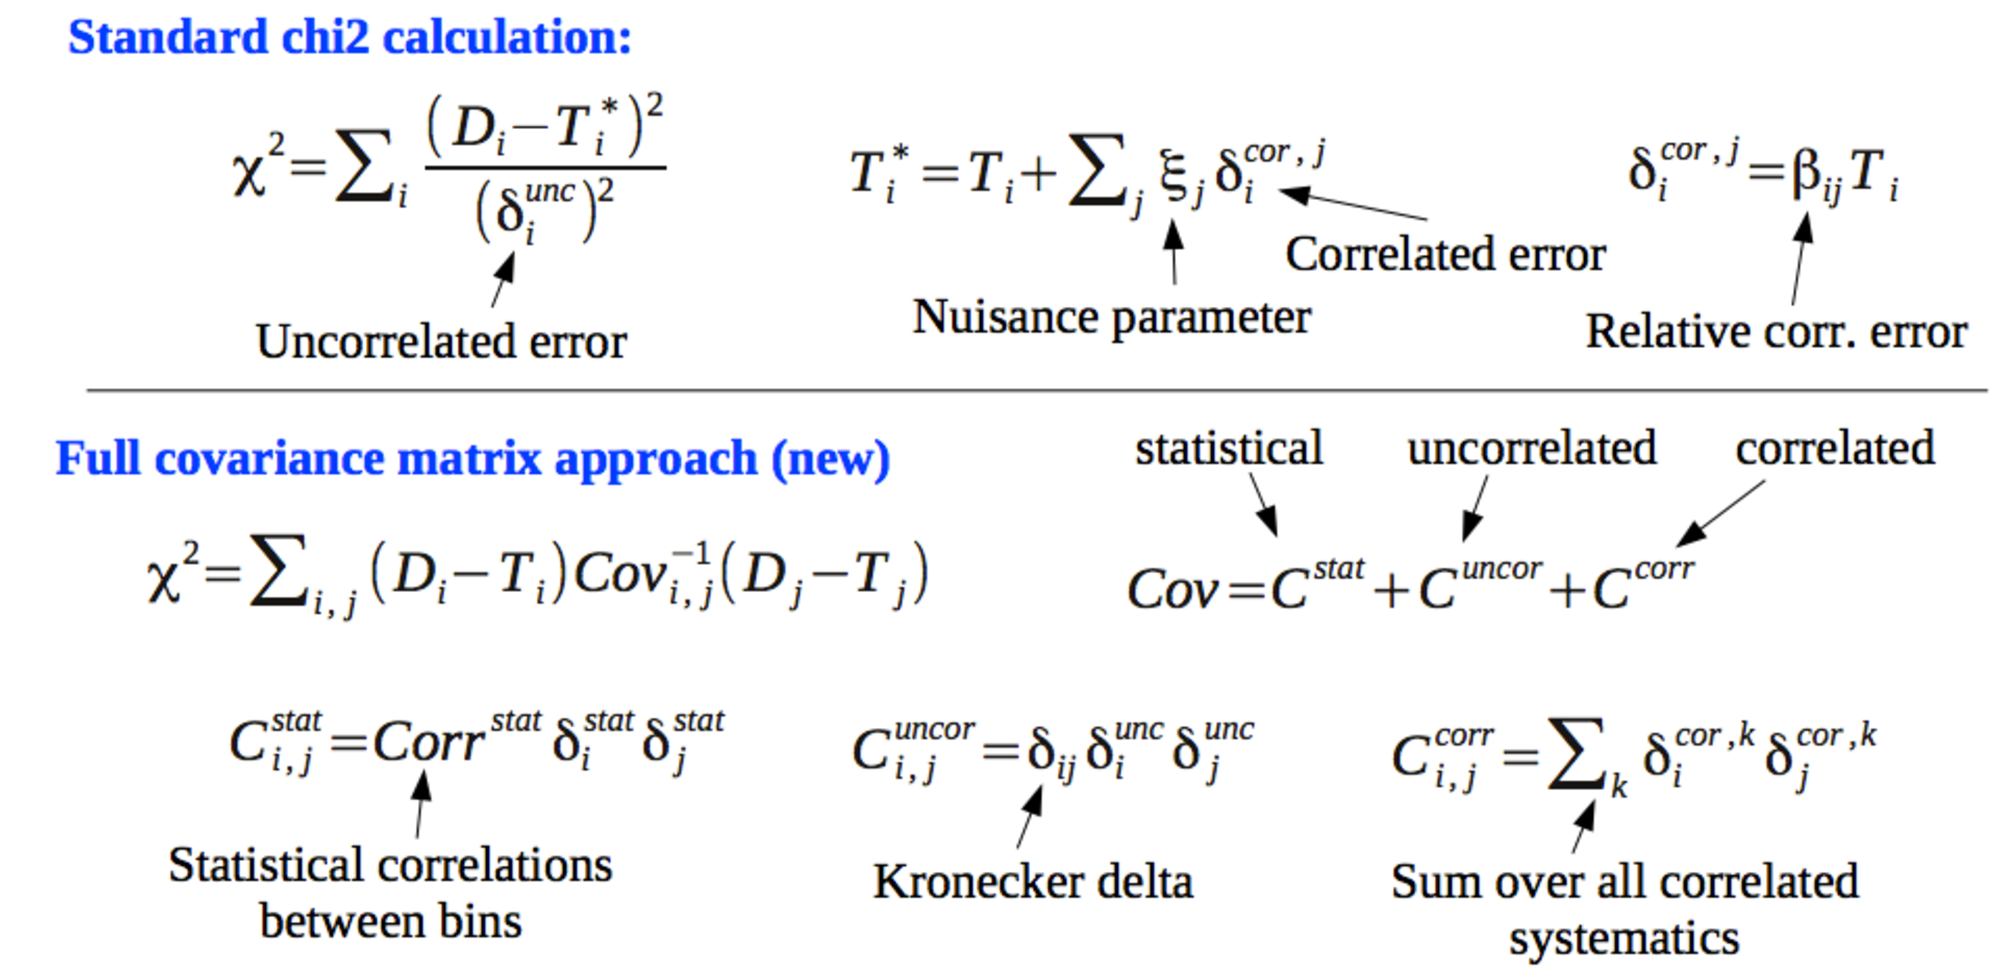
\includegraphics[width=0.75\linewidth]{figures/chi2.pdf}
\end{center}
\caption{Various $\chi^2$ representations in \fitter\ .}
\label{fig:chi2}
\end{figure}
The description starts with the most simple cases and extends to more evolved forms, which take into account possible biases 
arising from low statistics data. 

\subsubsection{Using Nuisance Parameters}
%%%%

In this subsection the focus is on the form of the $\chi^2$ using nuisance parameters. Different variants are discussed.


\begin{description}
%%%%
\item \bf{Simple Form} \rm

For a single data set, the $\chi^2$ function can be defined in a simple form 
\begin{equation}
 \chi^2_{\rm exp}\left(\boldsymbol{m},\boldsymbol{b}\right) = %\\
%~~~=
 \sum_i
 \frac{\left[m^i
- \sum_j \gamma^i_j m^i b_j  - {\mu^i} \right]^2}
{ \textstyle \left(\delta_{i,{\rm stat}}\mu^i\right)^2 +
\left(\delta_{i,{\rm uncor}}\,  \mu^i\right)^2}
 + \sum_j b^2_j.
\label{eq:ave}\end{equation}
%

\item \bf{Scaled Form} \rm

Equation~\ref{eq:ave} can be evolved as in~\cite{H1:2009bp}:

%
\begin{equation}
 \chi^2_{\rm exp}\left(\boldsymbol{m},\boldsymbol{b}\right) = %\\
%~~~=
 \sum_i
 \frac{\left[m^i
- \sum_j \gamma^i_j m^i b_j  - {\mu^i} \right]^2}
{ \textstyle \delta^2_{i,{\rm stat}}\mu^i \left(m^i -  \sum_j \gamma^i_j m^i b_j\right)+
\left(\delta_{i,{\rm uncor}}\,  m^i\right)^2}
 + \sum_j b^2_j + \mbox{\rm log penalty}
\label{eq:aven}\end{equation}
%
Here ${\mu^i}$ is the  measured central value  at a point $i$ 
with  relative statistical $\delta_{i,stat}$ 
and relative uncorrelated systematic uncertainty $\delta_{i,unc}$.
Further, 
%$\beta_j$ denotes a nuisance parameter for
% a correlated systematic error  source of type $j$ with an uncertainty while
$\gamma^i_j$ 
quantifies the sensitivity of the
measurement ${\mu^i}$ at the point $i$ to the systematic source $j$. 
The function $\chi^2_{\rm exp}$ depends on the set of
underlying physical quantities $m^i$ 
(denoted as the vector $\boldsymbol{m}$) and 
 the set of systematic uncertainties $b_j$ ($\boldsymbol{b}$).
This definition of the $\chi^2$ function takes into account that
systematic uncertainties are proportional to the central values 
(multiplicative errors), whereas the statistical errors scale 
with the square roots of the expected number of events. 
Other scaling properties for the statistical and uncorrelated
systematic uncertainties 
are discussed later.

\item \bf{Covariance Matrix} \rm

In the case of off-diagonal statistical uncertainties, the $\chi^2$ function
is
\begin{equation} \label{eq:chi2gen}
\chi^2_{\rm exp} (\boldsymbol{m},\boldsymbol{b}) = \sum_{ij} \left ( m^i - \sum_l \Gamma^i_l(m^i)b_l - \mu^i \right)
  C^{-1}_{{\rm stat.}~ij}(m^i,m^j) \left(  m^j - \sum_l \Gamma^j_l(m^j)b_l - \mu^j \right) + 
\sum_l b^2_l \,.
\end{equation}
Here the scaling properties of the correlated systematic uncertainties 
$\Gamma^i_j$ and
of the covariance matrix $C_{{\rm stat.}~ij}$ are expressed as a dependence
on $m_i$ and the dependence of $\delta_{\rm stat}$ on $b_j$ is ignored.

Eq.~\ref{eq:chi2gen} allows for two methods for fast determination
of the minimum, without need to include the formal nuisance parameters
corresponding to the systematic error sources into the minuit minimisation.
In the first method a minimisation vs. $b_j$ is used to define the covariance
matrix for the systematic uncertainties which is determined as
\begin{equation}
 C_{{\rm syst}~ij}= \sum_l \Gamma^i_l \Gamma^j_l \,.
\end{equation}
The total covariance matrix is given by the sum of the statistical and
systematic covariance matrices
\begin{equation} 
C_{{\rm tot}~ij} = C_{{\rm stat}~ij} + C_{{\rm syst}~ij}\,,
\end{equation}
and the $\chi^2$ function takes the form
\begin{equation}
  \chi^2( \boldsymbol{m}) = \sum_{ij} ( m^i - \mu^i) C^{-1}_{{\rm tot}~ij} 
( m^j - \mu^j)\,.
\end{equation}

The second method is used to determine optimal shifts of the nuisance
parameters at each iteration. The shifts are given by minimising 
Eq.~\ref{eq:chi2gen} vs. $b_l$, which leads to a system of  linear equations 
\begin{equation}
 \sum_k \sum_{ij} C^{-1}_{{\rm stat}~ij} \Gamma^i_l \Gamma^j_k \cdot b_k = \sum_{ij} C^{-1}_{{\rm stat}~ij} \Gamma^i_l (m^j - \mu^j)\,,
\end{equation}
where, $1\le l \le N_{\rm syst}$, the total number of correlated systematic uncertainties.

Finally the nuisance parameters $\boldsymbol{b}$ can be excluded from the $\chi^2$ minimisation.  
In this case, which is referred to as the Offset method, the minimum is determined for the values of $b$ set to zero
while uncertainties on the parameters $\boldsymbol{p}$ are determined by shifting each nuisance parameter $b_l$
by $\pm 1$. The total covariance matrix for parameters $p^i$ is determined as 
\begin{equation}
  C^{\rm Offset}_{ {\rm par}~ ij} = \sum_{l=1}^{N_{syst}} \Delta p^i_l \Delta p^j_l \,,
\end{equation}
where $ \Delta p^i_l = 0.5 ( p^i( b_l = +1 ) - p^i(b_l = -1))$ and the quality of the fit is estimated by 
fixing $\boldsymbol{p}$ to the values determined at the minimum and minimising with respect to $\boldsymbol{b}$

Finally, all three approaches can be combined together. For example, some of the systematic uncertainties
can be treated using the matrix method while others can be treated using the Hessian method. In this case, the
covariance matrix  $C_{\rm syst}$ is build using the corresponding sub-set of systematic sources and $C_{\rm stat}$ 
is replaced by $C_{\rm stat}+C_{\rm syst}$ in Eq.~\ref{eq:chi2gen}. Similarly, some of the systematic uncertainties
can be treated using Offset method and then $C^{\rm total}_{ {\rm par}} = C^{\rm Hessian}_{\rm par} + C^{\rm Offset}_{\rm par}$
where Offset and Hessian covariance matrices are calculated using corresponding systematic error sources.

\item \bf{Bias corrections}\rm

The correlated and uncorrelated systematic uncertainties can be treated as additive,  $\Gamma^i_l(m^i) = \gamma^i_l \mu^i$
or multiplicative, $\Gamma^i_l(m^i) = \gamma^i_l m^i$. A LogNormal treatment in which 
$ \mu^i + \sum_l \Gamma^i_j b_l$ is replaced by $ \mu^i \prod_l \exp( \gamma^i_j b_l) $ is foreseen for the
next release of the {\tt HERAFitter}. 

The statistical uncertainties can be treated as additive, $\Delta^i(m^i) = \delta^i \mu^i$  or as Poisson,
$\Delta^i(m^i) = \delta^i \sqrt{\mu^i m^i}$. More complex scaling from Eq.~\ref{eq:aven}, 
which depends on shifts of $b_j$, is implemented using an iterative approach: for the first iteration $b_l =0$ 
 is used to determine values of $b_l$ which are then applied in the second iteration. The statistical covariance
matrix is scaled in a similar manner. In this case the correlation matrix is assumed to be fixed, the diagonal
elements are updated using the prescription describe above and the covariance matrix is rescaled accordingly.

The modifications of the covariance matrix at each iteration of the minuit minimisation may lead to systematic
biases. There are two approaches that can be used to avoid these biases. In the first approach the covariance matrix is calculated
using the expected values at the first iteration of the minimisation and kept fixed to these values for further
iterations. This method requires several repetitions of the minimisation, to ensure that values close to optimal
are obtained already at the first iteration. The second method~\cite{h1:2012kk} modifies the $\chi^2$ function by adding a term
corresponding to a non constant value of the covariance matrix:
\begin{equation}
 \chi^2_{\rm log} = 2 \log \frac{\Delta^i(m^i)}{\Delta^i(\mu^i)} 
\end{equation}  
\end{description}


\subsubsection{\fitter\ implementation}
The form of the $\chi^2$ function and the scaling properties of the 
uncertainties are controlled globally by the {\sc CHI2SettingsName} and
{\sc  Chi2Settings} variables and individually using {\sc ``:''} modifiers.
The global scaling properties of the uncertainties are described in 
Table~\ref{tab:ErrScale}. The global form of the $\chi^2$ function
is defined by the {\sc CorChi2Type} parameter, see   
Table~\ref{tab:Chi2Type}.

The default behavior can be changed for each correlated systematic source by ``:'' modifiers.
They are described in Table~\ref{tab:SystModifier}. The modifiers should appear at the end 
of the systematic source name, e.g. {\sc 'H3:M'}. Several modifiers can be used, e.g. {\sc 'H3:M:C'}.

The names of systematic error sources are read first from the {\sc ListOfSources} variable of the 
{\sc \&Systematics} namelist, located in the {\sc steering.txt} file. Next the names are read from the
data files following the sequence given by the {\sc InputFileNames} list. The properties of each systematic
error source are defined by its first occurrence. That means that if, for example, {\sc 'H3:M:C'} is defined
in the {\sc ListOfSources} variable, the source {\sc 'H3'} is treated as multiplicative and using covariance
matrix approach regardless definitions in the data files. If, however, {\sc ListOfSources} defines a source
without any modifiers, e.g. {\sc 'H3'}, the default treatment, following the {\sc Chi2Settings} variable is
enforced for this source.
Thus the {\sc ListOfSources } variable is a convenient way to modify behavior of the correlated systematic
sources.

The shifts of the systematic sources are reported in the {\sc Results.txt} file. The uncertainty on the shift
is however estimated only approximately, neglecting the correlation with the theory parameters. An accurate determination
of the uncertainty can be achieved by using the toy MC method (see section~\ref{sec:ToyMC}) or by using {\sc ':E'} 
modifier. In the latter case the systematic source is treated using the {\tt Minuit} minimisation. Note, however,
that this approach can slow the minimisation convergence considerably.
\begin{table}
\begin{center}
\begin{tabular}{ccccc} 
\hline
{\sc CHI2SettingsName:}   & {\sc StatScale} & {\sc UncorSysScale} & {\sc CorSysScale} & Scaling rule \\
\hline
{\sc CHI2Settings}       &                 &                     &                   &              \\
\hline
  {\sc Poisson}   &  $+$  &  $+$  &  $-$  & $\sqrt{ m^i \mu^i}$ \\
  {\sc Linear}    & $-$   &  $+$  &  $+$  & $m^i$               \\
  {\sc NoRescale} & $+$   &  $+$  &  $+$  & $\mu^i$   \\
  {\sc LogNorm}   &  \multicolumn{4}{c}{Reserved, not implemented} \\
\hline
\end{tabular}
\end{center}
\caption{\label{tab:ErrScale}Global scaling rules for statistical, 
uncorrelated and correlated systematic uncertainties. The scaling
rule is given with respect to corresponding relative uncertainty.
E.g. for the {\sc Poisson} statistical uncertainty the absolute statistical
uncertainty is $\Delta_i = \delta_{i, {\rm stat}}\sqrt{m^i\mu^i}$   }
\end{table}

\begin{table}
\begin{center}
\begin{tabular}{cl}
\hline
    {\sc CorChi2Type} value &  Description \\
\hline
  {\sc Hessian}             & Use nuisance parameters.\\
  {\sc Matrix }             & Use covariance matrix. \\
  {\sc Offset }             & Use Offset method\\
\hline
\end{tabular}
\end{center}
\caption{\label{tab:Chi2Type}Possible values of the {\sc CorChi2Type} parameter which defines treatment of the correlated systematic uncertainties.}
\end{table}
 
\begin{table}
\begin{center}
\begin{tabular}{cl}
\hline
  Modifier &  Description \\
\hline
   \multicolumn{2}{c}{Scaling properties}\\
  {\sc :M}  &  Multiplicative scaling, $ m^i$ \\
  {\sc :A}  &  Additive scaling, $ \mu^i$ \\
  {\sc :P}  &  Poisson scaling, $ \sqrt{m^i\mu^i}$ \\
   \multicolumn{2}{c}{$\chi^2$ treatment}\\
  {\sc :N}  &  Nuisance parameter treatment \\
  {\sc :C}  &  Covariance matrix treatment \\
  {\sc :O}  &  Offset method treatment \\
  {\sc :E}  &  Nuisance parameter, included in {\sc Minuit} (``External'')\\
\hline
\end{tabular}
\end{center}
\caption{\label{tab:SystModifier}Modifiers for correlated systematic
uncertainty sources.}
\end{table}
% available as described in appendix~\ref{sec:herafitter}.
%%%%
%\subsubsection{Generalised Scaled Form}

%%%%%%%%%%%
%\subsection{Using Covariance Matrix}
%%%%%%%%%%%%%%%%%%%%%%%%%%%%%
